\section{MatTransform: Executable Soft-Chemistry Hypotheses}
\label{sec:mattransform}

A materials hypothesis becomes actionable when its intervention can be applied to an identified structure.  \mattransform provides a typed grammar that converts scientific proposals into deterministic operation plans.  The grammar distinguishes operations that create a child CIF from condition plans that describe an external or interfacial realization.  Both are retained in the candidate lineage.

\subsection{Structure operations and condition plans}

The implemented registry contains five structure operations: equivalent-site substitution, removal of an equivalent-site class, reasoned intercalation into a gap site, homogeneous strain, and reasoned layer sliding.  It also contains four condition or interface plans: carrier doping, electrostatic gating, magnetic proximity, and van der Waals heterostructure construction.  Figure~\ref{fig:softchem} summarizes the grammar.

\begin{figure}[t]
    \centering
    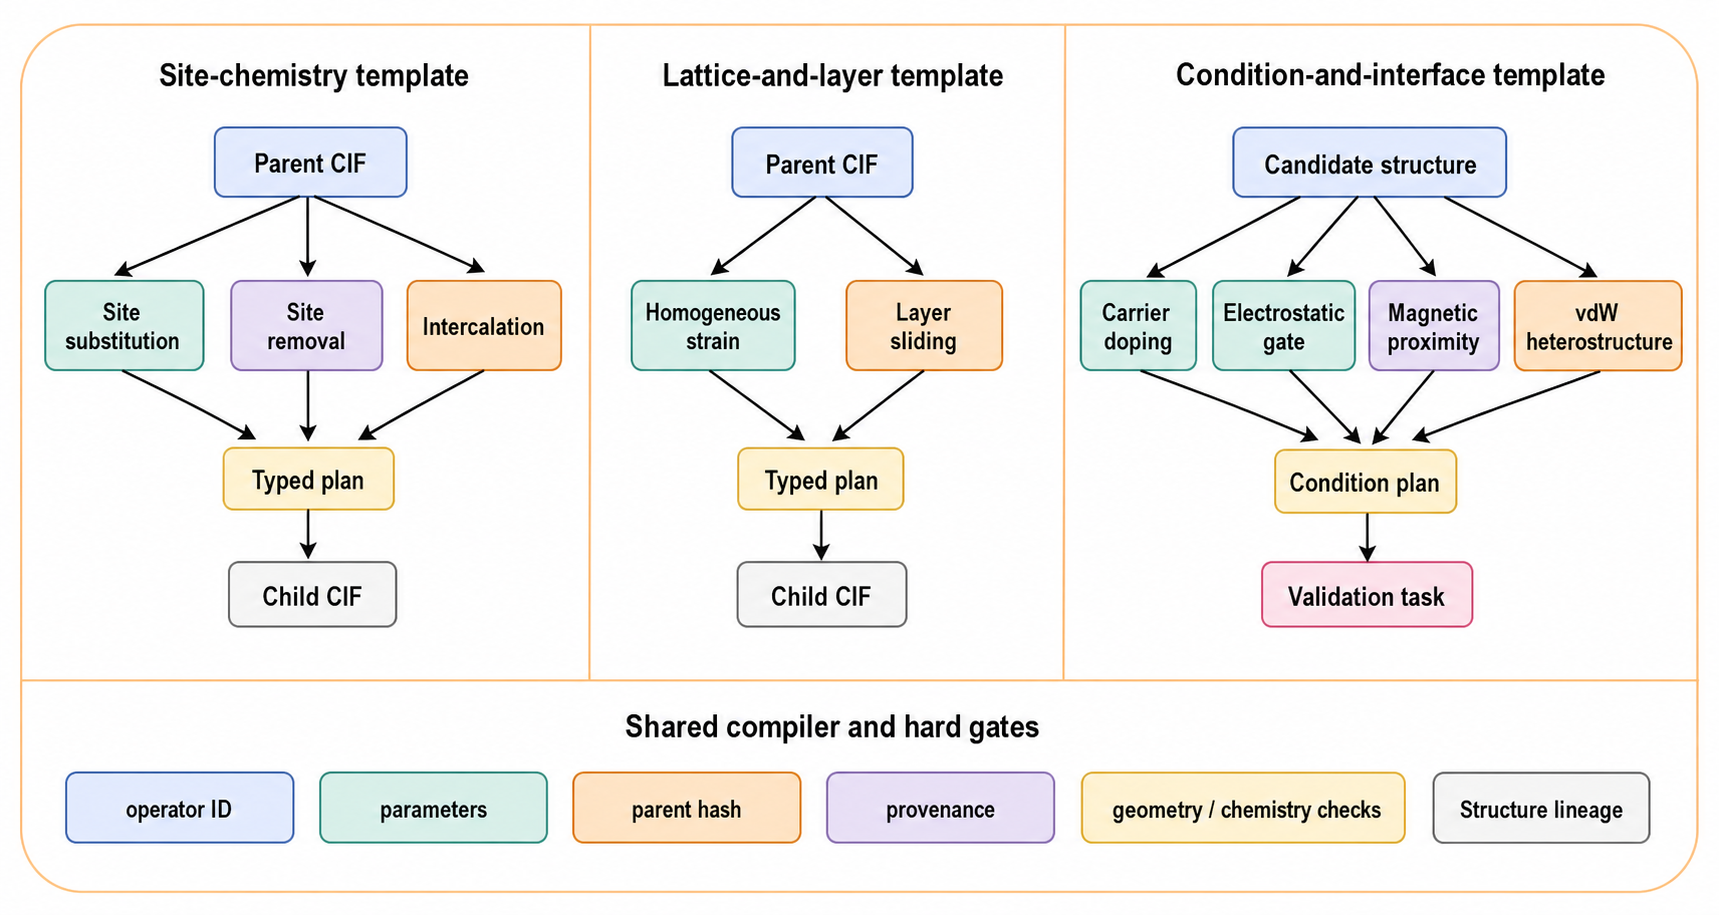
\includegraphics[width=\linewidth]{figures/softchem-grammar-image2-v2.png}
    \caption{\textbf{Stage-specific templates in the executable soft-chemistry grammar.}
    Site chemistry, lattice/layer changes, and condition/interface interventions use separate operator DAGs while sharing a typed compiler, content-hashed parent binding, provenance, and hard-gate layer.  Structure templates terminate in an explicit child CIF; condition templates terminate in a validation task.}
    \label{fig:softchem}
\end{figure}

An operation plan is represented as
\begin{equation}
    o=(\texttt{id},\texttt{version},s_{\mathrm{parent}},\theta,q,\pi),
\end{equation}
where $\theta$ is a typed parameter object, $q$ records the scientific rationale and target constraints, and $\pi$ is the provenance of the proposal.  The plan identifier is derived from canonical serialized content.  Replaying the same operator version and parameters on the same parent therefore recovers the same plan identity; changing the parent, parameters, or version produces a new lineage edge.

Equivalent-site substitution and removal act on a complete symmetry or equivalence class selected in the plan.  This makes site choice explicit and avoids a nominal composition change that has no crystallographic interpretation.  Intercalation stores both the species and the gap-site rationale.  Strain stores the deformation matrix, and layer sliding stores the selected layer and displacement vector.  Condition plans similarly retain carrier sign and concentration, gate geometry or field target, magnetic partner and interface orientation, or the components and registry of a heterostructure.

\begin{table}[t]
    \centering
    \caption{\textbf{MatTransform operator family.}}
    \label{tab:operators}
    \small
    \setlength{\tabcolsep}{3.8pt}
    \renewcommand{\arraystretch}{1.12}
    \begin{tabularx}{\linewidth}{>{\raggedright\arraybackslash}p{0.22\linewidth}>{\raggedright\arraybackslash}p{0.15\linewidth}XX}
        \toprule
        \normalfont\textbf{Operator} & \textbf{Output} & \textbf{Key frozen parameters} & \textbf{Typical scientific use} \\
        \midrule
        Site substitution & Child CIF & Site class, source and target species & Isoelectronic or aliovalent substitution; SOC and filling control \\
        Site-class removal & Child CIF & Site class and removal fraction encoded by the selected class & Vacancy or deintercalation route \\
        Gap-site intercalation & Child CIF & Species, gap and fractional position & Charge transfer or magnetic intercalation \\
        Homogeneous strain & Child CIF & Strain tensor and fixed-coordinate policy & Bandwidth, crossing and anisotropy tuning \\
        Layer sliding & Child CIF & Layer identity and displacement & Stacking and symmetry control \\
        Carrier doping & Condition plan & Carrier sign and target concentration & Fermi-level alignment and mixed filling \\
        Electrostatic gate & Condition plan & Field or charge target and geometry & Reversible filling or magnetic control \\
        Magnetic proximity & Interface plan & Magnetic partner and orientation & Exchange coupling without bulk substitution \\
        vdW heterostructure & Interface plan & Components, orientation and registry & Layer-selective topology and interface design \\
        \bottomrule
    \end{tabularx}
\end{table}

\subsection{Planning and deterministic execution}

The model proposes the scientific operation and explains why it addresses a particular constraint.  A deterministic planner resolves the proposal against the operator registry, validates the parameter schema, binds the exact parent artifact, and freezes the resulting plan.  Free text is not executed as a structure-editing instruction.  If the proposal cannot be resolved to an operator or lacks a required parameter, it remains a hypothesis and its missing realization is reported explicitly.

Execution is followed by hard-gate checks.  The child must parse and survive a canonical CIF round trip; composition and site counts must agree with the operator; fractional coordinates and lattice parameters must be finite; minimum interatomic distances must be physically admissible; and the intended dimensional or layer topology must not be destroyed by periodic-boundary artefacts.  Chemistry checks evaluate charge-balance or common-valence feasibility as a screening prior.  They constrain promotion but do not substitute for electronic-structure calculation.

The result stores the child structure, hard-gate verdicts, warnings, the parent and plan hashes, and the execution receipt.  A child that requires scientific review remains visible in the lineage together with the reason.  This is useful for open problems such as fractional substitution: an operator that replaces a complete O site class by F produces the explicit end member NbCl$_2$F, not a fictitious mixed NbO$_{1-x}$F$_x$Cl$_2$ structure.  The lineage makes the realized composition unambiguous and identifies partial occupancy or supercell enumeration as the next structure-design task.

\subsection{Lineages rather than isolated generations}

Generated structures are stored as edges in a directed acyclic lineage graph.  Each node is a content-addressed structure and each edge is an operation plan.  Multiple operations may share a parent, and successive operations form a route such as substitution $\rightarrow$ strain $\rightarrow$ gating.  Scientific observations attach to the structure node on which they were calculated.  Consequently, an encouraging parent band structure cannot be reported as evidence for an uncalculated child, and a child can inherit family-level rationale without inheriting its parent's numerical properties.
